\section{Background and Related Work}
\label{C++ Bad Forward Indirect Calls}

In the following, we provide a brief overview of the technical
concepts we use in the rest of this paper to detect and constrain 
forward and backward edges in program binaries as well as related work 
and our threat model.

% In this section,
% we present a brief overview of the concept of C++-based polymorphism in~\cref{Polymorphism in C++}
% and how indirect calls can be checked in practice in~\cref{C++ Indirect Calls in Practice}.
% In~\cref{section:countpolicy} we present a forward edge function parameter count-based policy (\cite{veen:typearmor}), and
% in~\cref{Security Implications of Forbidden Forward Indirect Calls} we highlight security implications of indirect calls ,while
% in~\cref{{Too Permissive Parameter-Based Policies}} we show that the state-of-the-art parameter count-based policy
% (\cref{section:countpolicy}) is imprecise w.r.t. to the enforced calltarget set per callsite. 
% Finally, in~\cref{Running Example: CVE X} we present in detail a real COOP attack.

% \subsection{Polymorphism in C++ Programs}
% % \textbf{Polymorphism in C++.}
% \label{Polymorphism in C++}
% Polymorphism, along inheritance and encapsulation, are the most used modern object-oriented concepts in C++. In C++, polymorphism allows accessing different types of objects 
% through a common base class. A pointer of the type of the base object can be used to point to object(s) which are derived from the base class. In C++, there are 
% several types of polymorphism:
% (a) compile-time (or static, usually is implemented with templates), 
% (b) runtime (dynamic, is implemented with inheritance and virtual functions), 
% (c) ad-hoc (\textit{e.g.,} if the range of actual types that can be used is finite and the combinations must be individually specified prior to use), and
% (d) parametric (\textit{e.g.,} if code is written without mention of any specific type and thus can be used transparently with any number of new types). 
% The first two are implemented through early and late binding, respectively. In C++, overloading concepts fall under the category of \textit{c)} and virtual functions, 
% templates or parametric classes fall under the category of pure polymorphism. However, C++ provides polymorphism through: 
% (i) virtual functions,
% (ii) function name overloading, and 
% (iii) operator overloading. 
% In this paper, we are concerned with dynamic polymorphism, based on virtual functions (see ISO/IEC N3690~\cite{iso:iecN3690}), because it can be exploited to call: 
% (x) illegitimate virtual table entries (not) contained in the class hierarchy by potentially varying the number of parameters and types,
% (y) legitimate virtual table entries (not) contained in the class hierarchy by potentially varying the number of parameters and types, and 
% (z) fake virtual tables entries not contained in the class hierarchy by potentially varying the number of parameters and types.
% By legitimate and illegitimate virtual table entries we mean those virtual table entries which for a single indirect callsite lie in the virtual table hierarchy. More 
% precisely, a virtual table entry is legitimate for a callsite if from the callsite to the virtual table containing the entry there is an inheritance path (see~\cite{haller:shrinkwrap}). 
% Virtual functions have several uses and issues associated, but for the scope of this paper we will look at the indirect callsites which are exploited by calling illegitimate virtual 
% table entries (\textit{i.e.,} functions) with varying number and type of parameters, see (x) above). More precisely, 
% (1) load-time enforcement: as calling each indirect callsite (\textit{i.e.,} callee) requires a fixed number of parameters which are passed each time the caller is calling, 
% we enforce a fine-grained CFI policy by statically determining the number and types of all function parameter that belong to an indirect callsite, and
% (2) runtime verification: as differentiating during runtime legitimate from illegitimate indirect caller/callee pairs requires parameter type and parameter number, we 
% insert before each indirect callsite a check used for determining during runtime if the caller matches with the callee based on certain CFI policies.

\newsavebox{\firstlisting}
\begin{lrbox}{\firstlisting}
\begin{minipage}[c]{\linewidth}
\begin{minted}[
% frame=lines,
framesep=2mm,
linenos,
%highlightlines={10},
highlightcolor={lightgray},
frame=none,
firstnumber=1,
framesep = 1.0cm,
linenos,
numbersep=2pt,
%gobble=2,
%frame=lines,
framesep=2mm,
fontsize=\tiny,      
% fontsize=\scriptsize,
% baselinestretch=1.2,
% bgcolor=LightGray,
% fontsize=\footnotesize,
]{C++}
class nsMultiplexInputStream final 
 :public nsIMultiplexInputStream //A0
 ,public nsISeekableStream //A1
 ,public nsIIPCSerializableInputStream //A2
 ,public nsICloneableInputStream{ //A3
nsTArray<nsCOMPtr<nsIInputStream>> mStreams;
NS_IMETHODIMP nsMultiplexInputStream::Close(){
  MutexAutoLock lock(mLock);
  mStatus = NS_BASE_STREAM_CLOSED;
  //set NS_OK flag
  nsresult rv = NS_OK;
  //get array length
  uint32_t len = mStreams.Length();
 //array-based main loop gadget (ML-G)
 for (uint32_t i = 0; i<len; ++i){
  //(0)hijacked object dispatch
  nsresult rv2=mStreams[i]->Close();
  if (NS_FAILED(rv2)) {
      rv = rv2;
  }
 }
  return rv;
}
\end{minted}
\end{minipage}
\end{lrbox}

% \subsubsection{Exploiting Object Dispatches in C++}
% % \textbf{Exploiting Object Dispatches.}
% \label{Exploiting Polymorphism Weaknesses}
%  \begin{figure}[!h]
%    \vspace{-.37cm}
%    \centering
%    \resizebox{2.3\linewidth}{!}{
%    \setlength{\unitlength}{0.1\textwidth}
%    \begin{picture}(10,4)
% %    \centering
%      \put(2.1, 1.5){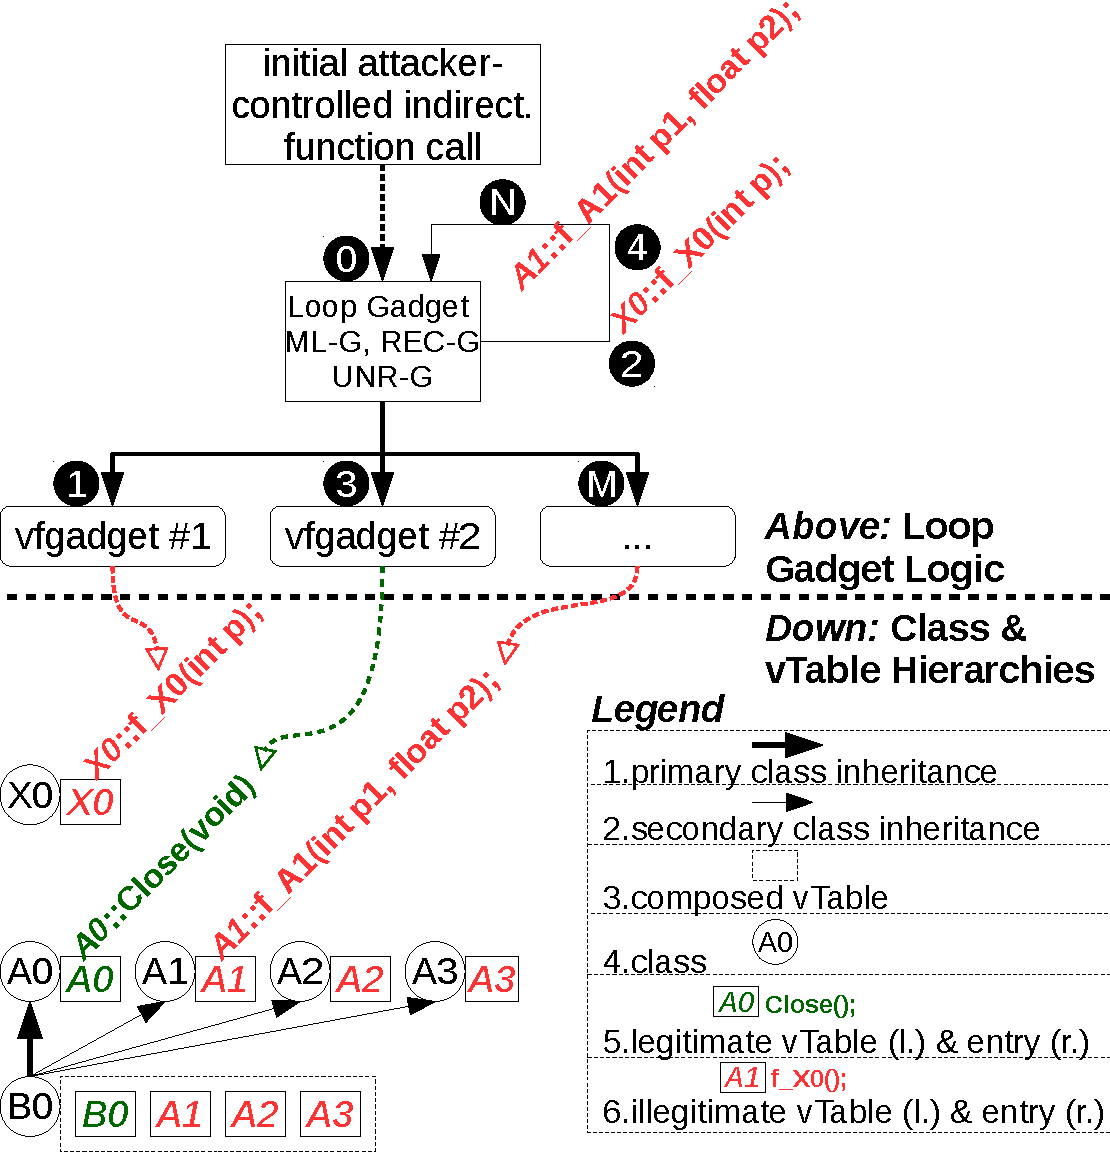
\includegraphics[width=.22\textwidth]{figures/loop.pdf}}
%      \put(.031, 2.5){\usebox{\firstlisting}}
%    \end{picture}}
% \vspace{-2.6cm}
% % \caption{Description of how a counterfeit object-oriented programming main loop gadget (ML-G) works.}
% \caption{COOP loop gadget (ML-G, REC-G, UNR-G) at work.}
% \label{Code example used to illustrate how a COOP loop gadget works}
% \end{figure}
% 
% Figure~\ref{Code example used to illustrate how a COOP loop gadget works}
% depicts a C++ code example (left) and how a COOP main-loop gadget (right) 
% (\textit{i.e.,} based either on ML-G (main-loop) or REC-G (recursive-gadget) or UNR-G (unrolled COOP gadget), 
% see~\cite{crane:readactor++} for more details) is used to sequentially call COOP gadgets by iterating trough 
% a loop (REC-G excluded) controlled by the attacker.
% 
% First, the object dispatch (see Figure~\ref{Code example used to illustrate how a COOP loop gadget works} line 17) is exploited by the attacker
% in order to call different functions in the whole program by iterating on an array of fake objects previously inserted in the array.
% 
% Second, in order to achieve this the attacker previously exploits an existing program memory corruption (\textit{e.g.,} buffer overflow) 
% which is further used to corrupt an object dispatch, \ding{182}, by inserting fake objects in the array and by changing the number of initial loop iterations.
% Next she invokes gadgets, \ding{182} and \ding{184} up to {\tiny\encircle{\Large{M}}}, 
% through the calls, \ding{183} and \ding{185} up to {\tiny\encircle{\Large{N}}}, contained in the loop. 
% As it can be observed in Figure~\ref{Code example used to illustrate how a COOP loop gadget works} she 
% can invoke from the same callsite legitimate functions (in total {\tiny\encircle{\Large{N}}}) residing in the virtual table (vTable) inheritance path
% (\textit{i.e.,} at the time of writing this paper this type of information is particularly hard to recuperate from program binaries)
% for this particular callsite, indicated with green color vTable entries. 
% However, a real COOP attack invokes illegitimate vTable entries residing in the whole initial program class hierarchy (or the extended one)
% with less or no relationship to the initial callsite,
% indicated with red-color vTable entries.
% 
% Third, in this way different addresses contained in the program (1) (vTable) hierarchy (contains only virtual members), 
% (2) class hierarchy (contains both virtual and non-virtual members) and (or) the whole program address space can be called. 
% For example the attacker can call in any entry in the:
% (1) class hierarchy of the whole program,
% (2) class hierarchy containing only legitimate targets for this callsite,
% (3) virtual table hierarchy of the whole program,
% (4) virtual table hierarchy containing only legitimate targets for this callsite,
% (5) virtual table hierarchy and class hierarchy containing only legitimate targets for this callsite, and
% (6) virtual table hierarchy and class hierarchy of the whole program.
% 
% Finally, because there are no intrinsic language semantics---such as object cast checks---in the C++ programming language for object dispatches
% the loop gadget indicated in Figure~\ref{Code example used to illustrate how a COOP loop gadget works} can be unconstrained used to call 
% any possible entry in the whole program. Thus, making any program address a gadget part.
% 
% \subsection{Type-Inference on Executables}
% \label{Type-Inference on Executables}
% Recovering variable types from executable programs
% is considered difficult in general, for two main reasons.
% First, the quality of the disassemble can vary considerably from the used underlying binary analysis
% framework to another and w.r.t. the compiler flags which were used to compile the binary.
% Note that a production binary can be more or less stripped (\textit{i.e.,} RTTI or other debugging symbols may or may not be available, etc.)
% from useful information which can be used during a type recovering analysis.
% \textsc{TypeShield} is based on DynInst and the quality of the executable disassembly is sufficient for our needs.
% For a more comprehensive review on the capabilities of DynInst and other tools we
% advice the reader to have a look at~\cite{andriesse:indepth}.
% Second, if the type inference analysis requires alias analysis then it is well known that 
% alias analysis in binaries is undecidable \cite{alias:undecidable} in theory and intractable 
% in practice~\cite{alan:mycroft}.
% Finally, there are several highly promising tools such as: Rewards~\cite{lin:rewards}, BAP~\cite{bap:brumley}, 
% SmartDec~\cite{fokin:smartdec}, and Divine~\cite{divine:balakrishnan}.
% These tools try with more or less success to recover (infer)
% type information from binary programs with different goals.
% Typical goals are: 
% (i) full program reconstruction (\textit{i.e.,} binary to code conversion, reversing, etc.), 
% (ii) checking for buffer overflows, and
% (iii) integer overflows and other types of memory corruptions.
% For a more exhaustive review of type inference recovering tools out of binaries we advice the reader
% to consult the following review~\cite{caballero:inference}.
% Interesting to notice is that the code from only a few of these tools is actually available.

% SmartDec seemed at first promising due to its simple type lattice that we wanted to leverage for our classification schema. 
% Its integration into our DynInst based environment was not successful mostly for several reasons, as it was deemed to 
% time consuming to extract the whole machinery and implement an interface to the DynInst disassembler.
% Therefore, we finally implemented our own version of function parameter type analysis and focused only
% on the wideness of the types, resulting in a simpler lattice than we initially intended.
% \vspace{-.25cm}
\subsection{Security Implications of Indirect Transfers}
% \textbf{Security Implications of Forbidden Indirect Calls.}
\label{Security Implications of Forbidden Forward Indirect Calls}
\textbf{Indirect Forward-Edge Transfers.} 
% The C++ language standard (N3690~\cite{iso:iecN3690}) does not specify what happens when calling different virtual table entries from an indirect callsite. 
% The standard says that we have a virtual function-related undefined behavior when: (citation) \textit{a virtual function call uses an explicit class member access and 
% the object expression refers to the complete object of x or one of that object's base class sub-objects but not x or one of its base class sub-objects}. As 
% undefined behavior is not a clearly defined concept, we argue that in order to be able to deal with undefined or unspecified behavior related to 
% virtual function calls one needs to know how these language-dependent concepts are implemented inside the used compilers.
Forbidden forward-edge indirect calls are the result of a virtual pointer (vPointer) corruption. A vPointer corruption is not a vulnerability, but rather a capability which
can be the result of a spatial or temporal memory corruption triggered by: 
(1) bad-casting~\cite{byoungyoung:typecasting} of C++ objects, 
(2) buffer overflow in a buffer adjacent to a C++ object or 
(3) a use-after-free condition~\cite{schuster:coop}.
A vPointer corruption can be exploited in several ways. A manipulated vPointer can be exploited by pointing it in any existing or added program virtual 
table entry or into a fake virtual table added by an attacker. For example, in case a vPointer
was corrupted, an attacker could highjack the control flow of the program and start a COOP attack~\cite{schuster:coop}.

vPointer corruptions are a real security threat that can be exploited if there is a memory corruption (\textit{e.g.,} buffer overflow), which is adjacent 
to the C++ object or a use-after-free condition. As a consequence, each corruption, which can reach an object (\textit{e.g.,} bad object casts), is a potential
exploit vector for a vPointer corruption. 

% Interestingly to notice in this context is that through:
% (1) memory layout analysis (through highly configurable compiler tool chains) of source code based locations which are highly prone to memory corruptions such 
% as declarations and uses of buffers, integers or pointer deallocations one can obtain the internal machine code layout representation;
% (2) analysis of a code corruption which is adjacent (based on (1)) to a C++ object based on application class hierarchy, the virtual table hierarchy and each
% location in source code where an object is declared and used (\textit{e.g.,} modern compiler tool chains can spill out this information for free), one can 
% derive an analysis which can determine---up to a certain extent---if a memory corruption can influence (\textit{e.g.,} is adjacent to) a C++ object.

% Finally, tools based on these two concepts (\textit{i.e.,} (1) and (2)) can be used by attackers, \textit{e.g.,} to find new vulnerabilities, and by defenders
% to harden the source code only at the places which are most exposed to such vulnerabilities (\textit{i.e.,} targeted security hardening).

\textbf{Indirect Backward-Edge Transfers.} 
Program backward edges (\textit{i.e.,} \texttt{jump}, \texttt{ret}, etc.) can be corrupted due to their provided indirection to assemble gadget chains in the following scenarios.
(1) No CFI protection technique was applied: In this case, the binary is not protected by any CFI policy. Obviously, the attacker can then hijack backward edges to \textit{jump} virtually 
anywhere in the binary in order to chain gadgets together.
(2) Coarse-grained CFI protected scenarios: In this scenario, if the attacker is aware of what addresses are protected and which are not through control flow bending, the attacker may deviate
the application flow to legitimate locations in order to link gadgets together.
(3) Fine-grained CFI protection scenarios: In this case, the legitimate target set is more strict than in (2) but still in this case, under the assumption that the attacker knows
which addresses are protected and which are not, he may be able through control flow bending to call legitimate targets, which are useful for assembling a gadget chain.
(4) Fully precise CFI protected scenarios (\textit{i.e.,} SafeStack \cite{volodymyr:cpi} based): In this scenario, the legitimate target set is more strict than in (3). Even though, we 
have a one-to-one mapping 
between calltargets and legitimate return sites, the attacker could theoretically use this one-to-one mapping to assemble gadget chains if at the legitimate calltarget return site there is a useful gadget. 
See \cite{carlini:bending} for more details about how control flow can be bent to legitimate addresses and how this is still dangerous in 
case that at the bent address location exists a useful gadget or even in fully CFI-complete scenarios. 

% 
% \subsection{Real COOP Attack Example}
% \label{Real COOP Attack Example}
% % \textbf{Real COOP Attack Example.}
% The bug CVE-2014-3176 was exploited by Crane \textit{et al.}~\cite{crane:readactor++} in order to perform a
% COOP attack, on the Google Chromium Web browser. The details of this attack are highly complex involving not properly 
% handled interaction of browser extensions between the IPC, the sync API, and Google V8 engine and for this reason we briefly present a better
% documented COOP exploit which is in principle similar with this attack.
% 
% \label{Running Example: CVE X}
% %%second pic
% \begin{figure}[h!]
%     \centering
%     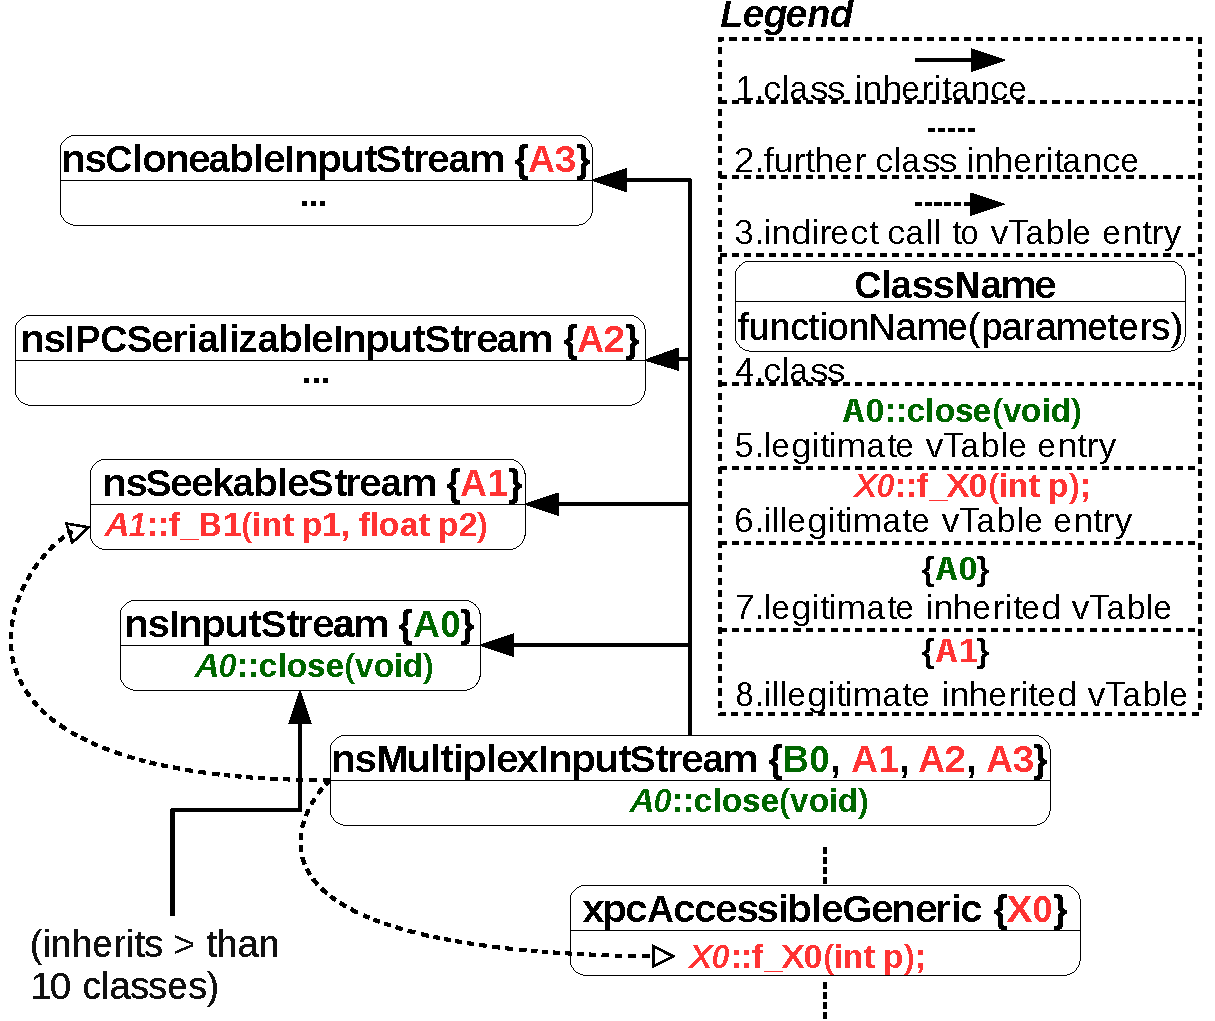
\includegraphics[width=0.35\textwidth]{figures/class_hierarchy.pdf}
% \caption{Class hierarchy of classes used in the COOP attack.}
% \label{Class exploit}
% \vspace{-.29cm}
% \end{figure}
% Figure~\ref{Class exploit} depicts~\footnote{The class inheritance hierarchy of the classes involved in the COOP attack against the Firefox browser. Red letters 
% indicate forbidden virtual table entries and green letters indicate allowed virtual table entries for the given indirect callsite
% contained in the main loop gadget.} a turing complete COOP attack~\cite{schuster:coop} which was used to attack the Mozilla Firefox Web browser. 
% By exploiting an existing buffer overflow bug the attacker was able to call into existing virtual table entries by having a main loop gadget at his disposal.
% 
% First, the attacker uses the C++ class \texttt{nsMultiplexInputStream} (see Figure~\ref{Class exploit}) which contains a 
% main loop gadget (ML-G) inside the \texttt{nsMultiplexInputStream::Close(void)} 
% function in order to perform indirect calls by dispatching calls on the fake objects contained in the array. The objects 
% contained in the array during normal execution are of \texttt{nsInputStream} type and each of the objects will call the 
% \texttt{Close(void)} function in order to close each of the previously opened streams. 
% 
% Second, for performing the COOP attack, the 
% attacker crafts a C++ program containing an array buffer holding six fake objects. These fake objects can call inside (and outside) 
% the initial class and virtual table hierarchies with no constraints. During the attack a buffer is created in order to hold the 
% fake objects. The crafted buffer will be used instead of the real code in order to call different functions available in the program code. 
% For example, the attacker calls a function contained in the class \texttt{xpcAccessibleGeneric} which is not in the class 
% hierarchy or virtual table hierarchy of the initially intended type of objects used inside the array. Moreover, the header 
% file of this class (\texttt{xpcAccessibleGeneric}) is not included in the class \texttt{nsMultiplex-InputStream}. 
% 
% Third, in total six fake objects are used to call into functions residing in unrelated class hierarchies with varying number of parameters 
% and return types. The final goal of this attack is to prepare the program memory such that a Unix shell can be opened at 
% the end of this attack.
% 
% 
% Finally, this example illustrates why detecting vPointer corruptions is not trivial for real-world applications. As depicted in 
% Figure~\ref{Class exploit}, the class \texttt{nsInputStream} has 11 classes which inherit directly or indirectly from 
% this class. The classes \texttt{nsSeekableStream}, \texttt{nsIPCSerializableInputStream} and \texttt{nsCloneableInputStream}
% provide additional inherited virtual tables which represent illegitimate calltargets for the initial \texttt{nsInputStream} 
% objects and legitimate calltargets for the six fake objects which were added during the attack. Furthermore, declaration and
% usage of the objects can be widely spread out in the source code. This makes detection of the object types 
% (\textit{i.e.,} base class), range of virtual tables (\textit{i.e.,} longest virtual table inheritance path for a
% particular callsite) and parameter types of the virtual table entries (\textit{i.e.,} functions) in which it is 
% allowed to call a trivial task for source code applications, but a hard task when one wants to apply similar 
% security policies (\textit{e.g.,} which rely on parameter types of virtual table entries) to binary executables.



%%%%Related Work
% \section{Related Work}
% \label{chapter:Related_Work}

% \subsection{Mitigation of Advanced CRAs}
% \textbf{Mitigation of Forward-Edge based Attacks.}
% \subsection{Mitigation of Forward-Edge based Attacks}
% \label{Mitigation of Advanced Code-Reuse Attacks}
% Recursive-COOP~\cite{crane:readactor++}, COOP~\cite{schuster:coop}, Subversive-C~\cite{subversive-c:lettner} and the attack of Lan \textit{et al.}~\cite{loop:oriented} are 
% forward-edge based CRAs which cannot be addressed with:
% (i)  shadow stacks techniques and hardware-based approaches such as Intel CET~\cite{intel:cet} (\textit{i.e.,} since advanced COOP do not violate 
% the caller/callee convention), 
% (ii) coarse-grained Control-Flow Integrity (CFI)~\cite{abadi:cfi2, abadi:cfi} techniques, and 
% (iii) OS-based approaches such as Windows Control Flow Guard~\cite{windows:cfguard} 
% since the precomputed CFG does not contain edges for indirect callsites which are explicitly exploited during the COOP attack.

% \subsubsection{Binary Based Techniques}
% The following tools address vTable protection through binary instrumentation, 
% but fail to mitigate against COOP: vfGuard~\cite{vfuard:aravind}, and vTint~\cite{vtint:zhang}.

% \subsubsection{Binary Based Forward-Edge Protection}
% TypeArmor~\cite{veen:typearmor} is a binary instrumentation tool that can protect against COOP.
% TypeArmor uses a fine-grained CFI policy based on caller/callee (but only indirect callsites) matching, which checks 
% during runtime if the number of provided and needed parameters match.
% \textsc{TypeShield} is related to TypeArmor~\cite{veen:typearmor}, since we also enforce strong binary-level 
% invariants on the number of function parameters. Further, \textsc{TypeShield} also aims for exclusive protection 
% against advanced exploitation techniques, which can bypass fine-grained CFI schemes and vTable protections at the 
% binary level. However, \textsc{TypeShield} offers a better restriction of calltargets to callsites, since we not 
% only restrict based on the number of parameters, but also on the width of their types. This results in much smaller 
% buckets that in turn can only target a smaller subset of all address-taken functions. 
%However, we rely for that on the variety of parameter types and when there is none, we will degrade into a parameter count policy.

% We are aware that there is still a long research path to go until binary based techniques can 
% recuperate program based semantic information from executable with the same precision as compiler based tools.
% This path could be even endless since compilers are optimized for speed and are designed to remove as much as possible semantic information
% from an executable in order to make the program run as fast as possible. In light of this fact,
% \textsc{TypeShield} is another attempt to recuperate just the needed semantic information (types and number of function parameters from
% indirect callsites) in order to be able to enforce a precise and with low overhead primitive against COOP attacks.

% VCI~\cite{vci:asiaccs} is a binary based tool (7.9\%) based on DynInst which can protect forward edge indirect control flow violations based 
% on reconstructing a quasi program class hierarchy (\textit{i.e.,} no class root node and the edges are not directed). The authors claim that 
% VCI is 10 times more precise w.r.t. reducing the calltarget set per callsite. In contrast to \textsc{TypeShield} VCI can not 
% protect backward-edge violations and we arguably due to the conservative analysis the VCI could skip some corner situations 
% allowing not legitimate calltargets.
% 
% Marx~\cite{marx} is most similar to VCI and as VCI this tool reconstructs the same type of quasi program class hierarchy. 
% No runtime efficiency numbers were provided in the paper.
% The authors claim that Marx can recuperate a class hierarchy which is more precise than that of IDAPro. The paper is geared towards
% first providing a tool which can be used by analyst in order to reverse engineer a binary. The precision of the calltarget set reduction
% per callsite should be similar to those of VCI but no comparison was compared in the paper. Compared to \textsc{TypeShield} 
% Marx can not protect against backward-edge violations and arguably has in common with VCI several limitations.

% VTPin~\cite{vtpin} is a runtime based tool ($\approx$5\%) used for protecting against VTable hijacking, via use-after-free vulnerabilities. VTPin pins
% all the freed VTable pointers on a safe VTable under VTPin’s control. For each object deallocation, VTPin deallocates all space allocated, but preserves and updates
% the VTable pointer with the address of the safe VTable. As consequence a dangling pointer can invoke 
% invoke a method provided by VTPin’s safe object. TPin needs to keep track of meta-data in order to detect runtime 
% dangling pointer violations. The tool can not protect against the COOP attack since the COOP attack does not rely on dangling pointers.
% In contrast with \textsc{TypeShield} this tool can not protect against backward-edges violations.

% In this paper, rather than claiming that the invariants offered by~\textsc{TypeShield} are sufficient
% to mitigate all versions of the COOP (as \cite{veen:typearmor} does) attack we conservatively claim that~\textsc{TypeShield} 
% further raises the bar w.r.t. what is possible when defending against COOP attacks on the binary level.

% \subsubsection{Source Code Based Techniques} Indirect callsite targets are checked based on vTable integrity.
% Different types of CFI policies are used such as in the following tools:
% SafeDispatch~\cite{safedispatch:jang}, IFCC/VTV~\cite{vtv:tice} LLVM and GCC compiler.
% Additionally, the Redactor++~\cite{crane:readactor++} uses randomization 
% vTrust~\cite{zhang:vtrust} checks calltarget function signatures, 
% CPI~\cite{volodymyr:cpi} uses a memory safety technique
% in order to protect against the COOP attack.
% 
% There are several source code based tools 
% which can successfully protect against the COOP attack.
% Such tools are: ShrinkWrap~\cite{haller:shrinkwrap}, IFCC/VTV~\cite{vtv:tice}, 
% SafeDispatch~\cite{safedispatch:jang}, vTrust~\cite{zhang:vtrust}, Readactor++~\cite{crane:readactor++}, CPI~\cite{volodymyr:cpi} and the
% tool presented by VTI~\cite{bounov:interleaving}. These tools profit from high precision
% since they have access to the full semantic context of the program trhough the scope
% of the compiler on which they are based. 
% Because of this reason, these tools target mostly other types of security problems than binary-based 
% tools address. For example, some of the last advancements in compiler based protection against code reuse attacks address mainly performance issues.
% Currently, most of the above presented tools are only forward edge enforcers of fine-grained CFI policies with 
% an overhead from 1\% up to 15\% (see \cite{cfi_survey_payer} for more details).
% 
% \subsubsection{Runtime Based Techniques}
% Several promising runtime-based defenses against advanced CRAs exist but currently none of them can successfully
% protect against the COOP attack.
% 
% IntelCET~\cite{intel:cet} is based on, \texttt{ENDBRANCH}, a new CPU instruction which can be used to enforce
% an efficient shadow stack mechanism. The shadow stack can be used to check during program execution if caller/return pairs match.
% Since the COOP attack reuses whole functions as gadgets and does not violate the caller/return convention than the 
% new feature provided by intel is useless in the face of this attack. Nevertheless, other highly notorious CRAs may not be possible
% after this feature will be implemented main stream in OSs and compilers.
% 
% Windows Control Flow Guard~\cite{windows:cfguard} is based on an user-space and kernel-space components which
% by working closely together can enforce an efficient fine-grained CFI policy based on a precomputed CFG.
% These new feature available in Windows 10 can considerably raise the bar for future attacks but in our opinion advanced CRAs
% such as COOP are still possible due the typical characteristics of COOP.
% 
% PathArmor~\cite{veen:cfi} is yet another tool which is based on a precomputed CFG and on the LBR register which can give a string of 16 up to
% 32 pairs of from/to addressed of different types of indirect instructions such as \texttt{call}, \texttt{ret}, and \texttt{jump}. 
% Because of the sporadic query of the LBR register (only during invocation of certain function calls) and because of the sheer amount of 
% data which passes through the LBR register this approach has in our opinion a fair potential to catch different types of CRAs but
% we think that against COOP this tool can be used only with limited success. 
% First, because of the fact that the precomputed CFG does not contain edges for all
% possible indirect callsites which are accessed during runtime. Second, the LBR buffer can be easily fooled by interleaving
% legitimate with illegitimate indirect callsites during the COOP attack.
% 
% % %maybe not relevant
% \subsection{Mitigation of not Advanced CRAs}
% \label{Mitigation of Code-Reuse Attacks}
% In the last couple of years researchers have provided many versions of new Code Reuse Attacks (CRAs).
% These new attacks were possible since DEP~\cite{dep} and ASLR~\cite{ASLR} were successfully bypassed mostly based
% on Return Oriented Programming (ROP)~\cite{ROP, kornau:rop, rop:shacham} on one hand and due to the discovery of 
% new exploitable hardware and software primitives, on the other hand.
% 
% ROP started to present itself in the last couple of years in many faceted ways such as:
% Jump Oriented Programming (JOP)~\cite{JOP1, JOP2, JOP3} which uses jumps in order to divert the control flow to the next gadget and 
% Call Oriented Programming (COP)~\cite{rop:carlini} which uses calls in order to chain gadgets together.
% CRAs have many manifestations and it is out of scope of this work to list them all.
% 
% First, CRAs can be mitigated in general in the following ways: 
% (i) binary instrumentation,
% (ii) source code recompilation and 
% (iii) runtime application monitoring.
% Second, there is a plethora of tools and techniques which try to enforce CFI based
% primitives in executables, source code and during runtime. Thus, we briefly
% present the solution landscape together with the approaches and the techniques on which these are based:
% (a) fine-grained CFI with hardware support, PathArmor~\cite{veen:cfi},
% (b) coarse-grained CFI used for binary instrumentation, CCFIR~\cite{ccfir:zhang},
% (c) coarse-grained CFI based on binary loader, CFCI~\cite{cfci:zhang}
% (d) fine-grained code randomization, O-CFI~\cite{mohan:opaque},
% (e) cryptography with hardware support, CCFI~\cite{ccfi:jose},
% (f) ROP stack pivoting, PBlocker~\cite{pblocker:prakash},
% (g) canary based protection, DynaGuard~\cite{dynaguard:petsios},
% (h) runtime and hardware support based on a combination of LBR, PMU and BTS registers CFIGuard~\cite{cfiguard:yuan}, and
% (i) source code recompilation with CFI and/or randomization enforcement against JIT-ROP attacks, MCFI~\cite{mcfi:niu}, 
% RockJIT~\cite{rockjit:niu} and PiCFI~\cite{perinput:niu}.
% 
% The above list is not exhaustive and new protection techniques can be obtained by combining available techniques
% or by using newly available hardware features or software exploits. However, notice that none of the above mentioned 
% techniques and tools can be used to mitigate COOP attacks.
% 

% \subsection{Mitigation of Backward-Edge based Attacks}
% Backward-Edge based code reuse attacks exploit the indirection provided by the return instructions 
% of a function. Usually each modern compiler builds caller/callee pairs by adhering to the so called caller-callee
% calling convention. This calling convention basically specifies that for each indirect call the return address of the function which returns after 
% it was called lies at the next address of the call instruction. 
% This calling convention is violated by all ROP attacks and also by 
% more recent advanced code reuse attacks. 
% Intel CET~\cite{intel:cet} is a promising technology from Intel in which the X86 instruction set is updated with new instructions (\textit{i.e.,} \texttt{END\_BRANCH}) instruction
% which should facilitate an efficient implementation of shadow stack implementations. Currently, this technology is not available and it is not foreseeable when this features will 
% be available in mass production.
% For brevity reasons we do not look herein into compiler and purely runtime techniques and advise the reader to look for 
% more details the following survey~\cite{cfi_survey_payer}.

% \subsubsection{Binary Based Techniques}
% \subsubsection{Binary Based Backward-Edge Protection}
% The CFI based implementation of Abadi et al.~\cite{abadi:cfi} is the first binary based implementation of a shadow stack.
% While at first glance promising, this implementation suffers from high performance overhead which is around 21\% due to the fact 
% that the inserted checks before each function return instruction are not runtime efficient. Further, this tool has high imprecision
% due to the fact that labels are reused and in this way not legitimate return addresses become legitimate, thus these 
% could be exploited by a skilled attacker.

% \subsubsection{Compiler Based Techniques}
% LLVM SafeStack~\cite{volodymyr:cpi} is a compiler based approach in which for each function stack a shadows stack copy is build with the help of the Clang compiler. These additional stacks
% are hidden by at least one level of indirection from the attacker such that she can not interfere with it. This approach is effective but suffers from a big binary blow-up which is not acceptable
% in any usage scenario. Currently, it was demonstrated that this implementation can be bypassed~\cite{safestack:bypassing}.
% 
% \subsubsection{Runtime Based Techniques}
% Windows CFGuard~\cite{windows:cfguard} is a technology by Microsoft deployed into Windows 8.1 and Windows 10. This technology allows to protect backward-edges by checking in a 
% shadow stack like fashion for backward-edge violations. The implementation is based on an interplay between user space and kernel space thus there is high potential that this 
% implementation is highly efficient even trough no official evaluation results are available.
% 
% PathArmor~\cite{veen:cfi} is a runtime based tool based on a Linux loadable module which can emulate shadow stack checks by using the \texttt{LBR} register which stores 
% callsite and target address pairs. The capacity of the LBR register is limited to 32 address pairs which can be stored. The tools sufferes from high runtime overhead and 
% it is imprecise since the address pairs can not be analyzed at the same speed as they arrive in this register. For this reason some pairs are skipped and thus the attacker has 
% the chance to mount and attack.



\subsection{Mitigation of Forward-Edge Based Attacks}
% \textbf{Checking Indirect Forward-Edge Calls in Practice.}
\label{C++ Indirect Calls in Practice}
Amongst \textbf{binary based tools}, TypeArmor~\cite{veen:typearmor}
($\approx$3\% runtime overhead) enforces a CFI-policy based on runtime checking of caller-callee pairs 
and function parameter count matching. Compared to \textsc{TypeShield}, this tool does not use function 
parameter types and assumes that a backward-edge protection is in place.
VCI~\cite{vci:asiaccs} and Marx~\cite{marx} are both based on approximated program class hierarchies: 
(1) do not recover the root class of the hierarchy, and (2) the edges between the classes are not oriented. Thus, both tools 
enforce for each callsite the same virtual table entry (\textit{i.e.,} index based) 
contained in one recovered class hierarchy denoted by father-child relationships between the recovered vtables. 
Finally, both tools use up to six heuristics and simplifying assumptions in order to make the problem of program
class hierarchy reconstruction tractable.

% \textbf{Source code based tools.} 
% To the best of our knowledge, only the Clang-CFI \cite{clang:cfi} and IFCC/VTV~\cite{vtv:tice} (up to 8.7\% performance overhead) compiler based tools are deployed in practice
% and can be used to check legitimate from illegitimate indirect forward-edge calls during runtime by checking if virtual object pointers comply with 
% the program class hierarchy inheritance relationships.
% Furthermore, ShrinkWrap~\cite{haller:shrinkwrap} is a GCC compiler based tool which further reduces the legitimate 
% virtual table ranges for a given indirect callsite (\textit{i.e.,} object dispatch) through precise analysis of the program class hierarchy and virtual table hierarchy. Evaluation results
% show similar performance overhead results as the previous mentioned tools but with more precision with respect to legitimate virtual table entries (calltargets) per callsite. 
% We noticed by analyzing the previous research results that the overhead incurred by these security checks can be very high due to the fact that for each callsite many range checks have to be
% performed during runtime. Therefore, in our opinion, despite its security benefit these types of checks are most likely not 
% applicable to software where performance is key.
% 
% \textbf{Other types of tools.} Other highly promising source code based tools (albeit also not deployed in practice) 
% which can overcome some of the drawbacks of the previously described tools are as follows. 
% Bounov \textit{et al.}~\cite{bounov:interleaving} presented a tool ($\approx$1\% runtime overhead)
% for indirect forward-edge callsite checking based on virtual table layout interleaving. The tool has better performance than VTV and better precision with
% respect to allowed virtual tables per indirect callsite. Its precision (selecting legitimate virtual tables for each callsite) compared to ShrinkWrap is
% lower since it does not consider virtual table inheritance paths. vTrust~\cite{zhang:vtrust} (average runtime overhead 2.2\%) enforces two layers of defense
% (virtual function type enforcement and virtual table pointer sanitization) against virtual table corruption, injection and reuse. 

\subsection{Mitigation of Backward-Edge Based Attacks}
\label{Mitigation of Return Edge Attacks}
According to one of the currently most comprehensive surveys~\cite{cfi:survey} assessing backward edge protection techniques and runtime overhead comparisons, tools can be distinguished into providing
 low, medium, and high levels of protection w.r.t. backward-edges. %Further, this survey 
%provides runtime overhead comparisons. 
%classifies the backward-edge protection techniques 
%in binary based, source code based, and other types (\textit{i.e.,} with HW support, etc.).

Specifically for \textbf{binary based tools}, the survey authors provide the following insights. The original CFI implementation 
from Abadi \textit{et al.}~\cite{abadi:cfi2} as well as MoCFI~\cite{mocfi}, 
kBouncer~\cite{kbouncer}, 
CCFIR~\cite{ccfir:zhang}, bin-CFI~\cite{mingwei:sekar}, O-CFI~\cite{mohan:opaque}, 
PathArmor~\cite{veen:cfi}, 
LockDown~\cite{payer:dimva} mostly suffer from imprecision (high number of reused labels); 
have low runtime efficiency; do not support shared libraries at all.

% \textbf{Source code based tools.} SafeStack~\cite{safestack}, Hypersafe~\cite{hypersafe}, CF-Locking~\cite{cflocking}, MIP~\cite{mip}, 
% CF-Restrictor~\cite{cfrestrictor}, KCoFi~\cite{kcocfi}, RockJIT~\cite{rockjit:niu}, CCFI~\cite{ccfi:jose}, 
% Kernel CFI~\cite{kernelcfi}, MCFI~\cite{mcfi:niu}, piCFI~\cite{perinput:niu} relatively high precision
% w.r.t. enforced address return set, and all do not support shared libraries (except MCFI), have high coverage (almost all backward edges are protected).
% 
% \textbf{Other types of tools.} ROPecker~\cite{ropecker}, HW-asst. CFI~\cite{davi:hardware}, 
% CFIGuard~\cite{cfiguard:yuan} are mostly relying on HW features which were not specifically built for protecting backward edges and 
% for this reason the tools are not runtime effective and their precision is rather low and mostly not effective against state of the art code
% reuse attacks.

\begin{center}
\begin{figure*}[t!]
\centering
   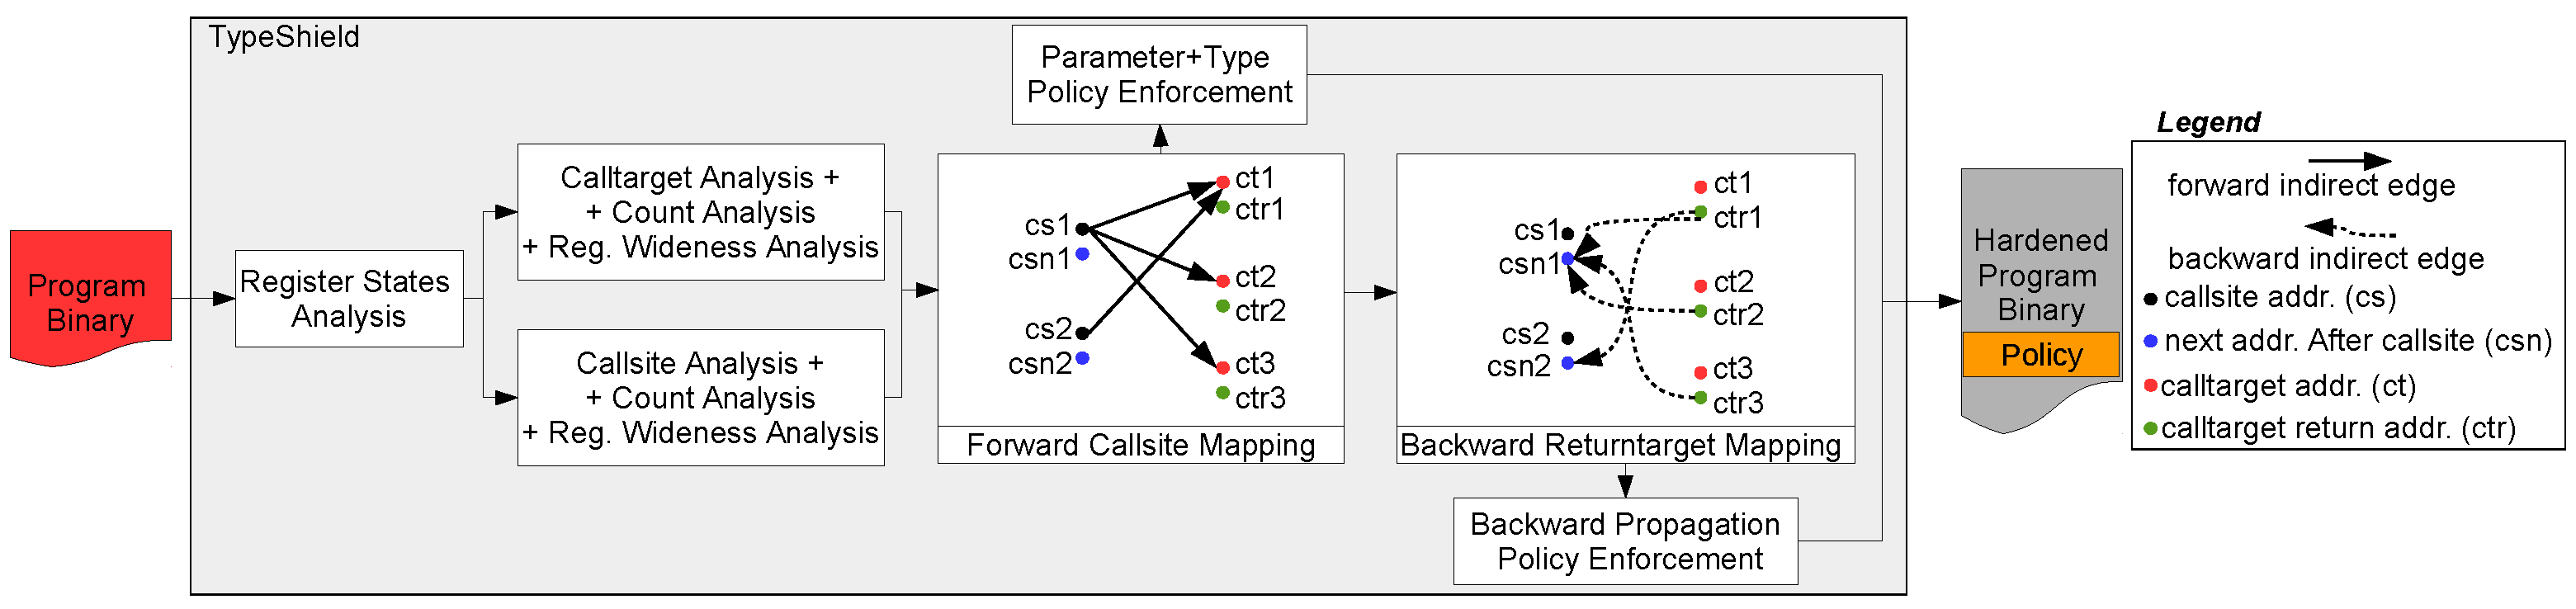
\includegraphics[width=.82\textwidth]{figures/overview.pdf}
   \vspace{-.25cm}
    \caption{Overview of the main steps performed by \textsc{TypeShield} when hardening a program binary.}
    \label{System overview.}
    \vspace{-.5cm}
 \end{figure*}
\end{center}
    \vspace{-.5cm}
\subsection{Threat Model}
\label{Adversary Model}

We align our threat model with the same basic assumptions as described in~\cite{veen:typearmor} w.r.t. the forward-edge.
More precisely, we assume a resourceful attacker that has read and write access to the data 
sections of the attacked program binary. We assume that the protected binary does not contain 
self-modifying code, handcrafted assembly or any kind of obfuscation. We also consider pages 
to be either writable or executable, but not both at the same time. Further, we assume 
that the attacker has the ability to exploit an existing memory corruption in order to hijack the program
control flow. 
As such, we consider a powerful, yet realistic adversary
model that is consistent with previous work on code-reuse
attacks and mitigations \cite{volodymyr:cpi}. 
The adversary is aware of the
applied defenses and has access to the source and non-randomized 
binary of the target application.
He can exploit (bend)
any backward-edge based indirect program transfer and
has the capability to make arbitrary memory writes. 
We assume that other forward-edge and backward-edge protection mechanisms
can be used in parallel with our techniques.
These defense
mechanisms are orthogonal to our protection policies. Our
approach does not rely on information hiding from the
attacker and as such we can tolerate arbitrary reads. 
Finally, the analyzed program binary is not hand-crafted and the compiler which was used
to generate the program binary adheres to one of the 
following most used caller-callee calling conventions \cite{arm:abi, microsoft:abi, itanium:abi}.


